\chapter{Number of Stops}
    In this chapter we will derive the expected number of stops for particular arrangments of the machine. The machine is wired to stop when $\overline\sigma$ has cycle type other than $(26)$. Turing only considers what he calls \textbf{normal stops} during his calculation of the expected number of stops. This is a stop which has cycle-type $(25,1)$.
    We will attempt to expand to a consideration of all possible stops. 
    \subsection{Prior Work}
    \subsection{Stops Without Diagonal Board}
    \begin{center}
        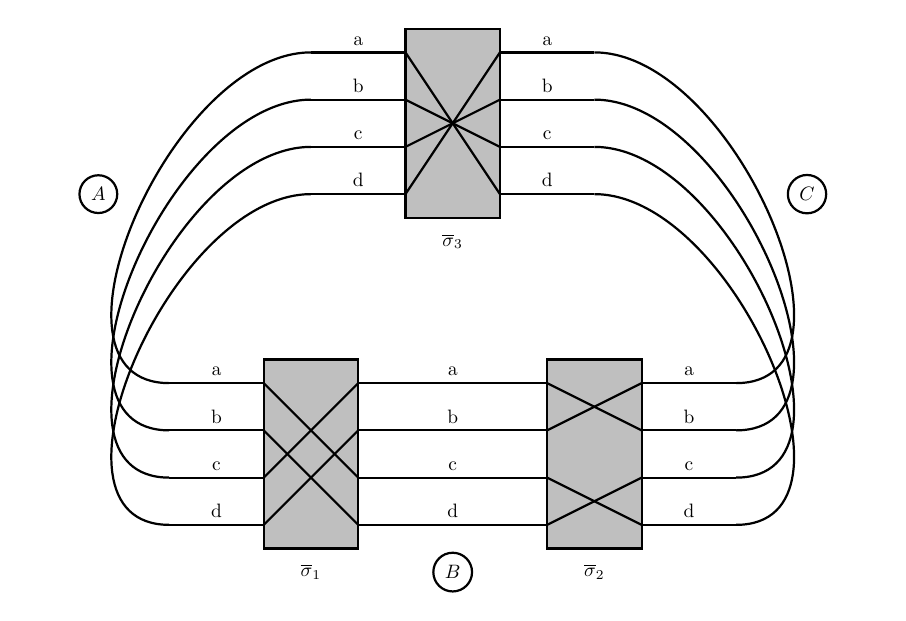
\begin{tikzpicture}[thick, scale=0.6, every node/.style={scale=0.7}]
            % Draw the box
            \draw[fill=lightgray] (2,-1.5) rectangle (4,2.5) node[midway] {};
            
            \node at (3, -2) {$\overline\sigma_3$};

            % Draw the wires entering the box
            \draw[-] (0, 2) -- (2, 2) node[midway, above] {a};
            \draw[-] (0, 1) -- (2, 1) node[midway, above] {b};
            \draw[-] (0, 0) -- (2, 0) node[midway, above] {c};
            \draw[-] (0,-1) -- (2,-1) node[midway, above] {d};

            % Draw the wires exiting the box with crossed mappings
            \draw[-] (4, 2) -- (6,2) node[midway, above] {a};
            \draw[-] (4, 1) -- (6, 1) node[midway, above] {b};
            \draw[-] (4, 0) -- (6, 0) node[midway, above] {c};
            \draw[-] (4,-1) -- (6, -1) node[midway, above] {d};

            % Draw the lines inside the box to represent the mapping
            \draw[-] (2, 2) -- (4,-1);
            \draw[-] (2, 1) -- (4, 0);
            \draw[-] (2, 0) -- (4, 1);
            \draw[-] (2,-1) -- (4, 2);

            \draw[-] (0-3, 2-7) to[out=180, in=180] (0, 2) node[midway, above] {};
            \draw[-] (0-3, 1-7) to[out=180, in=180] (0, 1) node[midway, above] {};
            \draw[-] (0-3, 0-7) to[out=180, in=180] (0, 0) node[midway, above] {};
            \draw[-] (0-3, -1-7) to[out=180, in=180] (0, -1) node[midway, above] {};

            \draw[-] (6+3, 2-7) to[out=360, in=360] (6, 2) node[midway, above] {};
            \draw[-] (6+3, 1-7) to[out=360, in=360] (6, 1) node[midway, above] {};
            \draw[-] (6+3, 0-7) to[out=360, in=360] (6, 0) node[midway, above] {};
            \draw[-] (6+3, -1-7) to[out=360, in=360] (6, -1) node[midway, above] {};

            \draw[fill=lightgray] (2-3,-1.5-7) rectangle (4-3,2.5-7) node[midway] {};

            \node at (3-3, -2-7) {$\overline\sigma_1$};

            % Draw the wires entering the box
            \draw[-] (0-3, 2-7) -- (2-3, 2-7) node[midway, above] {a};
            \draw[-] (0-3, 1-7) -- (2-3, 1-7) node[midway, above] {b};
            \draw[-] (0-3, 0-7) -- (2-3, 0-7) node[midway, above] {c};
            \draw[-] (0-3,-1-7) -- (2-3,-1-7) node[midway, above] {d};

            % Draw the wires exiting the box
            \draw[-] (4-3, 2-7) -- (6-3,2-7) node[right, above] {a};
            \draw[-] (4-3, 1-7) -- (6-3, 1-7) node[right, above] {b};
            \draw[-] (4-3, 0-7) -- (6-3, 0-7) node[right, above] {c};
            \draw[-] (4-3,-1-7) -- (6-3, -1-7) node[right, above] {d};

            % Draw the lines inside the box to represent the mapping
            \draw[-] (2-3, 2-7) -- (4-3, 0-7);
            \draw[-] (2-3, 1-7) -- (4-3, -1-7);
            \draw[-] (2-3, 0-7) -- (4-3, 2-7);
            \draw[-] (2-3,-1-7) -- (4-3, 1-7);

            \draw[fill=lightgray] (2+3,-1.5-7) rectangle (4+3,2.5-7) node[midway] {};
            
            \node at (3+3, -2-7) {$\overline\sigma_2$};


            % Draw the wires entering the box
            \draw[-] (0+3, 2-7) -- (2+3, 2-7) node[midway, above] {};
            \draw[-] (0+3, 1-7) -- (2+3, 1-7) node[midway, above] {};
            \draw[-] (0+3, 0-7) -- (2+3, 0-7) node[midway, above] {};
            \draw[-] (0+3,-1-7) -- (2+3,-1-7) node[midway, above] {};

            % Draw the wires exiting the box
            \draw[-] (4+3, 2-7) -- (6+3,2-7) node[midway, above] {a};
            \draw[-] (4+3, 1-7) -- (6+3, 1-7) node[midway, above] {b};
            \draw[-] (4+3, 0-7) -- (6+3, 0-7) node[midway, above] {c};
            \draw[-] (4+3,-1-7) -- (6+3, -1-7) node[midway, above] {d};

            \draw[-] (2+3, 2-7) -- (4+3, 1-7);
            \draw[-] (2+3, 1-7) -- (4+3, 2-7);
            \draw[-] (2+3, 0-7) -- (4+3, -1-7);
            \draw[-] (2+3,-1-7) -- (4+3, 0-7);

            \node[draw,circle] at (-4.5, -1) {$A$};
            \node[draw,circle] at (3, -9) {$B$};
            \node[draw,circle] at (10.5, -1) {$C$};



        \end{tikzpicture}
    \end{center}
    Consider our simple example of a loop of three Enigmas on four letters. We might expect that $\overline\sigma = \overline\sigma_3\overline\sigma_2\overline\sigma_1$ being generated
    from considerably random permutations, is itself a random permutation. If this is the case then we would expect that we would get a $(4)$ cycle with a probability of $\frac{1}{4}$. Then we expect the machine to stop
    with probability $\frac{3}{4}$. With enough loops this probability decreases exponentially and the machine has a tractible number of stops. 
    However, try as we may, we can never find a collection of Enigma permutations $\{\overline\sigma_1, \overline\sigma_2, \overline\sigma_3\}$ which generate a $(4)$ cycle in $\overline\sigma$. This is to say, in our above arrangment, the 
    machine will stop at \emph{every} rotor position thus making the process of checking stops intractible. 
    \\\\To see why this is the case, note that each $\overline\sigma_i$ has cycle type $(2,2)$ thus they are permutations of even parity. On the other hand, any $(4)$ cycle will have odd parity. 
    When we compose $3$ even permutations (i.e. $\overline\sigma_3\overline\sigma_2\overline\sigma_1$) we will always get an even parity permutation, thus this resulting permutation can \emph{never} be a $(4)$ cycle. 
    \\\\In the case of the Bombe, a cycle of even length can never produce a permutation with a $(26)$ cycle. We can emperically observe this by simulating the Bombe's operation on a cycle of length $8$ and we find that every single rotor
    position produces a stop. 
    \\\\From the above it is clear that $\overline\sigma$ is certainly not a purely random permutation, and simulations of loops of Enigma permutations of various lengths show that the probability distribution of these permutations is highly dependent on 
    the length of the loop. A table for estimated probabilities for Enigma machines on $4$ letters is shown below. 
    \\\\NOTE THAT WE ARE ASSUMING AN ENIGMA MACHINE IS A RANDOM 2,2... CYCLE
    \\\\Given how skewed the distribution of permutations are for each cycle length it follows naturally that to express the probability of a stop with a particular machine arrangement should not just be a function 
    of the number of closures or letters in a menu, but rather the particular length of each closure.
    \subsubsection{Singular Loop}\text{}
    \\\\For the case of a single loop we can run a simulation to estimate the probability of a stop given the length of a loop. This is akin to the table above though we combine the total probabilities of any cycle type other than $(26)$ to get a probability of a stop
    for each length of loop. 
    \subsubsection{Multiple Loops}\text{}
    \\\\Multiple loops presents some complexities. Initally one might suspect that these loops are independent, and while the cycle type probabilities of each loop may be independent, due to the electrical interconnections between the loops we need to take more into account. 
    For example, we have noted that an even loop length of Enigma machines will always stop. However, two loops of odd length may result in a configuration that will not cause a stop. To see this consider our example on $4$ letters. In this case, an odd length loop can never generate a $(4)$ cycle. 
    Consider now the following loops of Enigma permutations representing permutations $\overline\sigma$ and $\overline\delta$ respectively.
    \subsection{Introducing the Diagonal Board}
    \begin{center}
        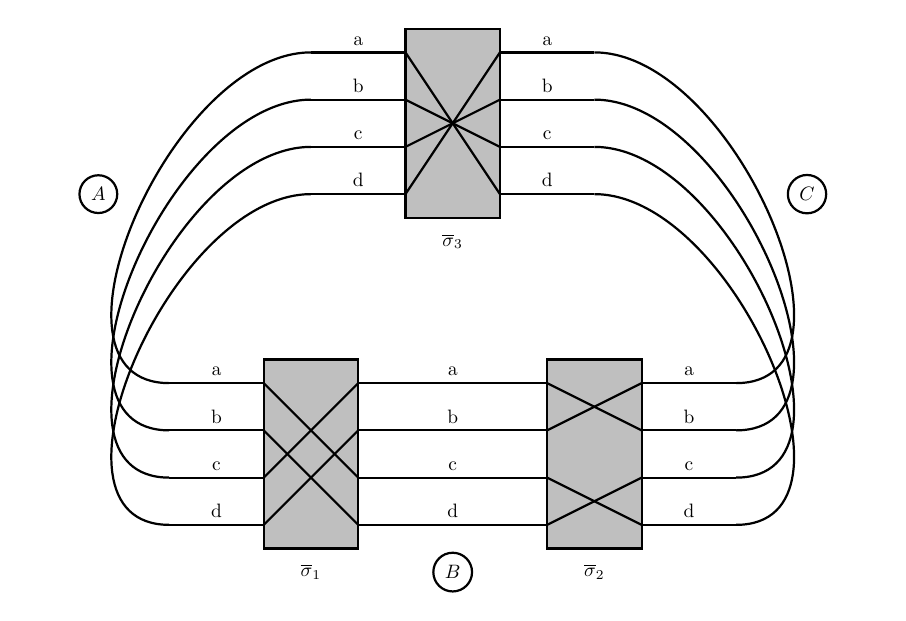
\begin{tikzpicture}[thick, scale=0.6, every node/.style={scale=0.7}]
            % Draw the box
            \draw[fill=lightgray] (2,-1.5) rectangle (4,2.5) node[midway] {};
            
            \node at (3, -2) {$\overline\sigma_3$};

            % Draw the wires entering the box
            \draw[-] (0, 2) -- (2, 2) node[midway, above] {a};
            \draw[-] (0, 1) -- (2, 1) node[midway, above] {b};
            \draw[-] (0, 0) -- (2, 0) node[midway, above] {c};
            \draw[-] (0,-1) -- (2,-1) node[midway, above] {d};

            % Draw the wires exiting the box with crossed mappings
            \draw[-] (4, 2) -- (6,2) node[midway, above] {a};
            \draw[-] (4, 1) -- (6, 1) node[midway, above] {b};
            \draw[-] (4, 0) -- (6, 0) node[midway, above] {c};
            \draw[-] (4,-1) -- (6, -1) node[midway, above] {d};

            % Draw the lines inside the box to represent the mapping
            \draw[-] (2, 2) -- (4,-1);
            \draw[-] (2, 1) -- (4, 0);
            \draw[-] (2, 0) -- (4, 1);
            \draw[-] (2,-1) -- (4, 2);

            \draw[-] (0-3, 2-7) to[out=180, in=180] (0, 2) node[midway, above] {};
            \draw[-] (0-3, 1-7) to[out=180, in=180] (0, 1) node[midway, above] {};
            \draw[-] (0-3, 0-7) to[out=180, in=180] (0, 0) node[midway, above] {};
            \draw[-] (0-3, -1-7) to[out=180, in=180] (0, -1) node[midway, above] {};

            \draw[-] (6+3, 2-7) to[out=360, in=360] (6, 2) node[midway, above] {};
            \draw[-] (6+3, 1-7) to[out=360, in=360] (6, 1) node[midway, above] {};
            \draw[-] (6+3, 0-7) to[out=360, in=360] (6, 0) node[midway, above] {};
            \draw[-] (6+3, -1-7) to[out=360, in=360] (6, -1) node[midway, above] {};

            \draw[fill=lightgray] (2-3,-1.5-7) rectangle (4-3,2.5-7) node[midway] {};

            \node at (3-3, -2-7) {$\overline\sigma_1$};

            % Draw the wires entering the box
            \draw[-] (0-3, 2-7) -- (2-3, 2-7) node[midway, above] {a};
            \draw[-] (0-3, 1-7) -- (2-3, 1-7) node[midway, above] {b};
            \draw[-] (0-3, 0-7) -- (2-3, 0-7) node[midway, above] {c};
            \draw[-] (0-3,-1-7) -- (2-3,-1-7) node[midway, above] {d};

            % Draw the wires exiting the box
            \draw[-] (4-3, 2-7) -- (6-3,2-7) node[right, above] {a};
            \draw[-] (4-3, 1-7) -- (6-3, 1-7) node[right, above] {b};
            \draw[-] (4-3, 0-7) -- (6-3, 0-7) node[right, above] {c};
            \draw[-] (4-3,-1-7) -- (6-3, -1-7) node[right, above] {d};

            % Draw the lines inside the box to represent the mapping
            \draw[-] (2-3, 2-7) -- (4-3, 0-7);
            \draw[-] (2-3, 1-7) -- (4-3, -1-7);
            \draw[-] (2-3, 0-7) -- (4-3, 2-7);
            \draw[-] (2-3,-1-7) -- (4-3, 1-7);

            \draw[fill=lightgray] (2+3,-1.5-7) rectangle (4+3,2.5-7) node[midway] {};
            
            \node at (3+3, -2-7) {$\overline\sigma_2$};


            % Draw the wires entering the box
            \draw[-] (0+3, 2-7) -- (2+3, 2-7) node[midway, above] {};
            \draw[-] (0+3, 1-7) -- (2+3, 1-7) node[midway, above] {};
            \draw[-] (0+3, 0-7) -- (2+3, 0-7) node[midway, above] {};
            \draw[-] (0+3,-1-7) -- (2+3,-1-7) node[midway, above] {};

            % Draw the wires exiting the box
            \draw[-] (4+3, 2-7) -- (6+3,2-7) node[midway, above] {a};
            \draw[-] (4+3, 1-7) -- (6+3, 1-7) node[midway, above] {b};
            \draw[-] (4+3, 0-7) -- (6+3, 0-7) node[midway, above] {c};
            \draw[-] (4+3,-1-7) -- (6+3, -1-7) node[midway, above] {d};

            \draw[-] (2+3, 2-7) -- (4+3, 1-7);
            \draw[-] (2+3, 1-7) -- (4+3, 2-7);
            \draw[-] (2+3, 0-7) -- (4+3, -1-7);
            \draw[-] (2+3,-1-7) -- (4+3, 0-7);

            \node[draw,circle] at (-4.5, -1) {$A$};
            \node[draw,circle] at (3, -9) {$B$};
            \node[draw,circle] at (10.5, -1) {$C$};



        \end{tikzpicture}
        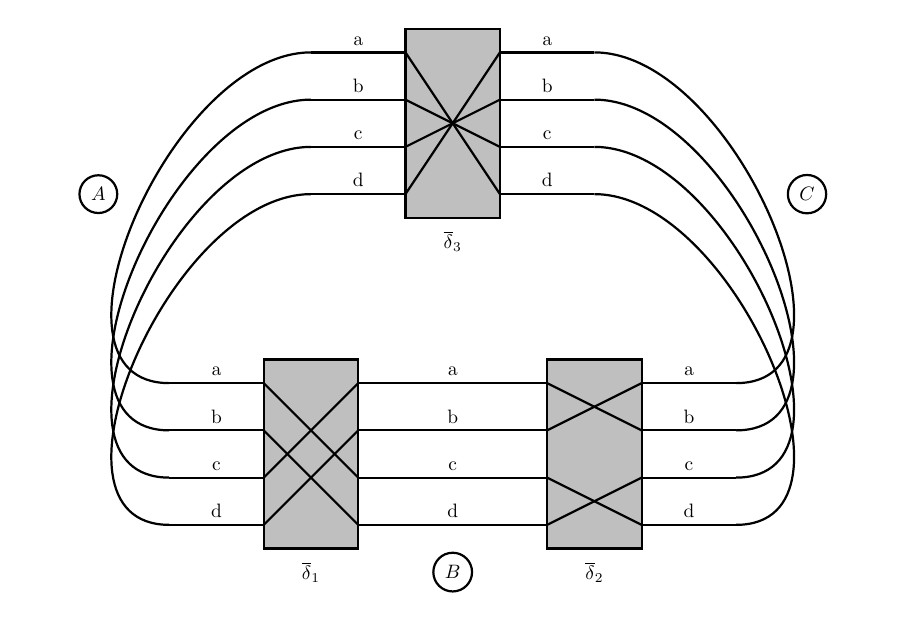
\begin{tikzpicture}[thick, scale=0.6, every node/.style={scale=0.7}]
            % Draw the box
            \draw[fill=lightgray] (2,-1.5) rectangle (4,2.5) node[midway] {};
            
            \node at (3, -2) {$\overline\delta_3$};

            % Draw the wires entering the box
            \draw[-] (0, 2) -- (2, 2) node[midway, above] {a};
            \draw[-] (0, 1) -- (2, 1) node[midway, above] {b};
            \draw[-] (0, 0) -- (2, 0) node[midway, above] {c};
            \draw[-] (0,-1) -- (2,-1) node[midway, above] {d};

            % Draw the wires exiting the box with crossed mappings
            \draw[-] (4, 2) -- (6,2) node[midway, above] {a};
            \draw[-] (4, 1) -- (6, 1) node[midway, above] {b};
            \draw[-] (4, 0) -- (6, 0) node[midway, above] {c};
            \draw[-] (4,-1) -- (6, -1) node[midway, above] {d};

            % Draw the lines inside the box to represent the mapping
            \draw[-] (2, 2) -- (4,-1);
            \draw[-] (2, 1) -- (4, 0);
            \draw[-] (2, 0) -- (4, 1);
            \draw[-] (2,-1) -- (4, 2);

            \draw[-] (0-3, 2-7) to[out=180, in=180] (0, 2) node[midway, above] {};
            \draw[-] (0-3, 1-7) to[out=180, in=180] (0, 1) node[midway, above] {};
            \draw[-] (0-3, 0-7) to[out=180, in=180] (0, 0) node[midway, above] {};
            \draw[-] (0-3, -1-7) to[out=180, in=180] (0, -1) node[midway, above] {};

            \draw[-] (6+3, 2-7) to[out=360, in=360] (6, 2) node[midway, above] {};
            \draw[-] (6+3, 1-7) to[out=360, in=360] (6, 1) node[midway, above] {};
            \draw[-] (6+3, 0-7) to[out=360, in=360] (6, 0) node[midway, above] {};
            \draw[-] (6+3, -1-7) to[out=360, in=360] (6, -1) node[midway, above] {};

            \draw[fill=lightgray] (2-3,-1.5-7) rectangle (4-3,2.5-7) node[midway] {};

            \node at (3-3, -2-7) {$\overline\delta_1$};

            % Draw the wires entering the box
            \draw[-] (0-3, 2-7) -- (2-3, 2-7) node[midway, above] {a};
            \draw[-] (0-3, 1-7) -- (2-3, 1-7) node[midway, above] {b};
            \draw[-] (0-3, 0-7) -- (2-3, 0-7) node[midway, above] {c};
            \draw[-] (0-3,-1-7) -- (2-3,-1-7) node[midway, above] {d};

            % Draw the wires exiting the box
            \draw[-] (4-3, 2-7) -- (6-3,2-7) node[right, above] {a};
            \draw[-] (4-3, 1-7) -- (6-3, 1-7) node[right, above] {b};
            \draw[-] (4-3, 0-7) -- (6-3, 0-7) node[right, above] {c};
            \draw[-] (4-3,-1-7) -- (6-3, -1-7) node[right, above] {d};

            % Draw the lines inside the box to represent the mapping
            \draw[-] (2-3, 2-7) -- (4-3, 0-7);
            \draw[-] (2-3, 1-7) -- (4-3, -1-7);
            \draw[-] (2-3, 0-7) -- (4-3, 2-7);
            \draw[-] (2-3,-1-7) -- (4-3, 1-7);

            \draw[fill=lightgray] (2+3,-1.5-7) rectangle (4+3,2.5-7) node[midway] {};
            
            \node at (3+3, -2-7) {$\overline\delta_2$};


            % Draw the wires entering the box
            \draw[-] (0+3, 2-7) -- (2+3, 2-7) node[midway, above] {};
            \draw[-] (0+3, 1-7) -- (2+3, 1-7) node[midway, above] {};
            \draw[-] (0+3, 0-7) -- (2+3, 0-7) node[midway, above] {};
            \draw[-] (0+3,-1-7) -- (2+3,-1-7) node[midway, above] {};

            % Draw the wires exiting the box
            \draw[-] (4+3, 2-7) -- (6+3,2-7) node[midway, above] {a};
            \draw[-] (4+3, 1-7) -- (6+3, 1-7) node[midway, above] {b};
            \draw[-] (4+3, 0-7) -- (6+3, 0-7) node[midway, above] {c};
            \draw[-] (4+3,-1-7) -- (6+3, -1-7) node[midway, above] {d};

            \draw[-] (2+3, 2-7) -- (4+3, 1-7);
            \draw[-] (2+3, 1-7) -- (4+3, 2-7);
            \draw[-] (2+3, 0-7) -- (4+3, -1-7);
            \draw[-] (2+3,-1-7) -- (4+3, 0-7);

            \node[draw,circle] at (-4.5, -1) {$A$};
            \node[draw,circle] at (3, -9) {$B$};
            \node[draw,circle] at (10.5, -1) {$C$};



        \end{tikzpicture}
    \end{center}

    \begin{center}
        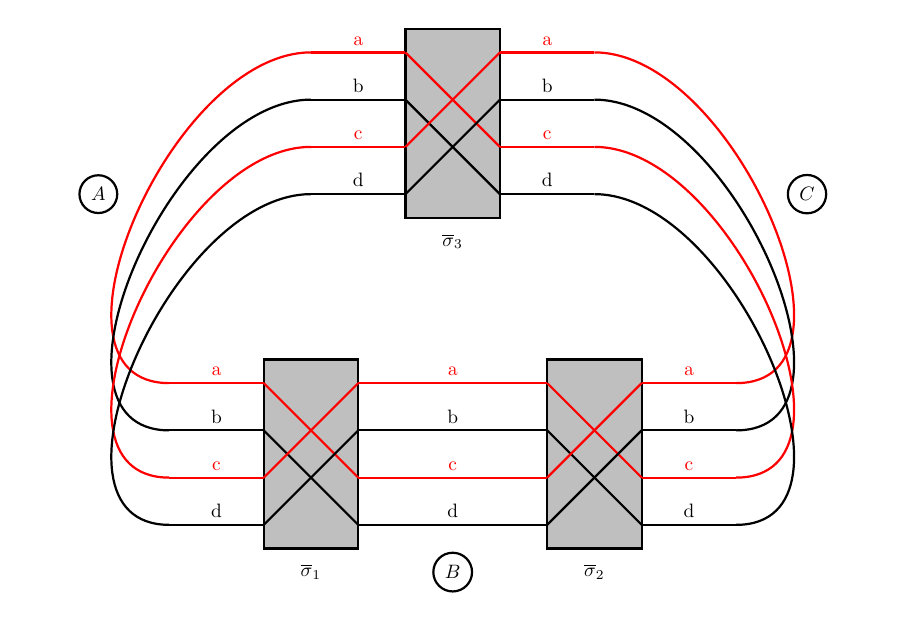
\begin{tikzpicture}[thick, scale=0.6, every node/.style={scale=0.7}]
            % Draw the box
            \draw[fill=lightgray] (2,-1.5) rectangle (4,2.5) node[midway] {};
            
            \node at (3, -2) {$\overline\sigma_3$};

            % Draw the wires entering the box
            \draw[-, red] (0, 2) -- (2, 2) node[midway, above] {a};
            \draw[-] (0, 1) -- (2, 1) node[midway, above] {b};
            \draw[-, red] (0, 0) -- (2, 0) node[midway, above] {c};
            \draw[-] (0,-1) -- (2,-1) node[midway, above] {d};

            % Draw the wires exiting the box with crossed mappings
            \draw[-, red] (4, 2) -- (6,2) node[midway, above] {a};
            \draw[-] (4, 1) -- (6, 1) node[midway, above] {b};
            \draw[-, red] (4, 0) -- (6, 0) node[midway, above] {c};
            \draw[-] (4,-1) -- (6, -1) node[midway, above] {d};

            % Draw the lines inside the box to represent the mapping
            \draw[-, red] (2, 2) -- (4,0);
            \draw[-] (2, 1) -- (4, -1);
            \draw[-, red] (2, 0) -- (4, 2);
            \draw[-] (2,-1) -- (4, 1);

            \draw[-, red] (0-3, 2-7) to[out=180, in=180] (0, 2) node[midway, above] {};
            \draw[-] (0-3, 1-7) to[out=180, in=180] (0, 1) node[midway, above] {};
            \draw[-, red] (0-3, 0-7) to[out=180, in=180] (0, 0) node[midway, above] {};
            \draw[-] (0-3, -1-7) to[out=180, in=180] (0, -1) node[midway, above] {};

            \draw[-, red] (6+3, 2-7) to[out=360, in=360] (6, 2) node[midway, above] {};
            \draw[-] (6+3, 1-7) to[out=360, in=360] (6, 1) node[midway, above] {};
            \draw[-, red] (6+3, 0-7) to[out=360, in=360] (6, 0) node[midway, above] {};
            \draw[-] (6+3, -1-7) to[out=360, in=360] (6, -1) node[midway, above] {};

            \draw[fill=lightgray] (2-3,-1.5-7) rectangle (4-3,2.5-7) node[midway] {};

            \node at (3-3, -2-7) {$\overline\sigma_1$};

            % Draw the wires entering the box
            \draw[-, red] (0-3, 2-7) -- (2-3, 2-7) node[midway, above] {a};
            \draw[-] (0-3, 1-7) -- (2-3, 1-7) node[midway, above] {b};
            \draw[-, red] (0-3, 0-7) -- (2-3, 0-7) node[midway, above] {c};
            \draw[-] (0-3,-1-7) -- (2-3,-1-7) node[midway, above] {d};

            % Draw the wires exiting the box
            \draw[-, red] (4-3, 2-7) -- (6-3,2-7) node[right, above] {a};
            \draw[-] (4-3, 1-7) -- (6-3, 1-7) node[right, above] {b};
            \draw[-, red] (4-3, 0-7) -- (6-3, 0-7) node[right, above] {c};
            \draw[-] (4-3,-1-7) -- (6-3, -1-7) node[right, above] {d};

            % Draw the lines inside the box to represent the mapping
            \draw[-, red] (2-3, 2-7) -- (4-3, 0-7);
            \draw[-] (2-3, 1-7) -- (4-3, -1-7);
            \draw[-, red] (2-3, 0-7) -- (4-3, 2-7);
            \draw[-] (2-3,-1-7) -- (4-3, 1-7);

            \draw[fill=lightgray] (2+3,-1.5-7) rectangle (4+3,2.5-7) node[midway] {};
            
            \node at (3+3, -2-7) {$\overline\sigma_2$};


            % Draw the wires entering the box
            \draw[-, red] (0+3, 2-7) -- (2+3, 2-7) node[midway, above] {};
            \draw[-] (0+3, 1-7) -- (2+3, 1-7) node[midway, above] {};
            \draw[-, red] (0+3, 0-7) -- (2+3, 0-7) node[midway, above] {};
            \draw[-] (0+3,-1-7) -- (2+3,-1-7) node[midway, above] {};

            % Draw the wires exiting the box
            \draw[-, red] (4+3, 2-7) -- (6+3,2-7) node[midway, above] {a};
            \draw[-] (4+3, 1-7) -- (6+3, 1-7) node[midway, above] {b};
            \draw[-, red] (4+3, 0-7) -- (6+3, 0-7) node[midway, above] {c};
            \draw[-] (4+3,-1-7) -- (6+3, -1-7) node[midway, above] {d};

            \draw[-, red] (2+3, 2-7) -- (4+3, 0-7);
            \draw[-] (2+3, 1-7) -- (4+3, -1-7);
            \draw[-, red] (2+3, 0-7) -- (4+3, 2-7);
            \draw[-] (2+3,-1-7) -- (4+3, 1-7);

            \node[draw,circle] at (-4.5, -1) {$A$};
            \node[draw,circle] at (3, -9) {$B$};
            \node[draw,circle] at (10.5, -1) {$C$};
        \end{tikzpicture}
        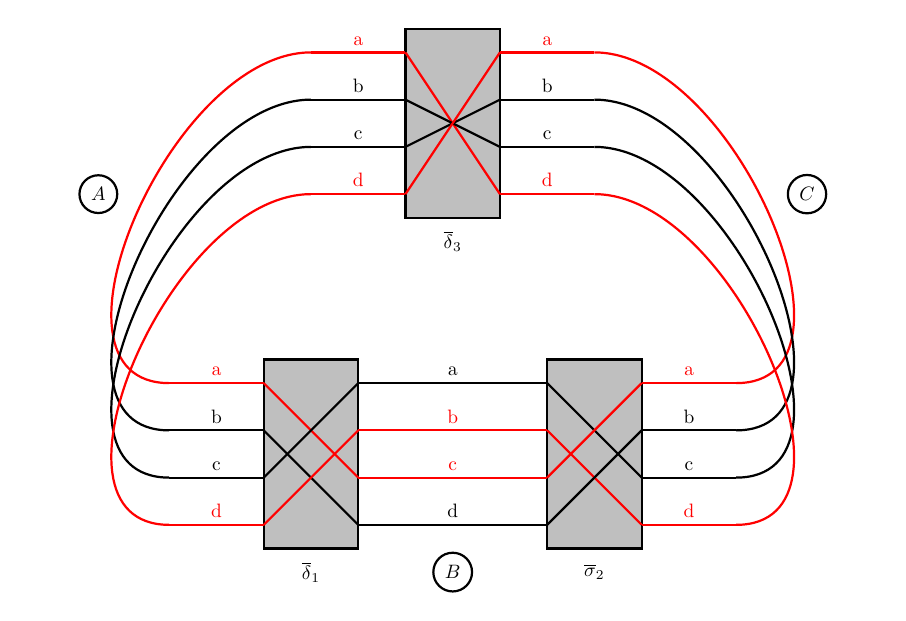
\begin{tikzpicture}[thick, scale=0.6, every node/.style={scale=0.7}]
            % Draw the box
            \draw[fill=lightgray] (2,-1.5) rectangle (4,2.5) node[midway] {};
            
            \node at (3, -2) {$\overline\delta_3$};

            % Draw the wires entering the box
            \draw[-, red] (0, 2) -- (2, 2) node[midway, above] {a};
            \draw[-] (0, 1) -- (2, 1) node[midway, above] {b};
            \draw[-] (0, 0) -- (2, 0) node[midway, above] {c};
            \draw[-, red] (0,-1) -- (2,-1) node[midway, above] {d};

            % Draw the wires exiting the box with crossed mappings
            \draw[-, red] (4, 2) -- (6,2) node[midway, above] {a};
            \draw[-] (4, 1) -- (6, 1) node[midway, above] {b};
            \draw[-] (4, 0) -- (6, 0) node[midway, above] {c};
            \draw[-, red] (4,-1) -- (6, -1) node[midway, above] {d};

            % Draw the lines inside the box to represent the mapping
            \draw[-, red] (2, 2) -- (4,-1);
            \draw[-] (2, 1) -- (4, 0);
            \draw[-] (2, 0) -- (4, 1);
            \draw[-, red] (2,-1) -- (4, 2);

            \draw[-, red] (0-3, 2-7) to[out=180, in=180] (0, 2) node[midway, above] {};
            \draw[-] (0-3, 1-7) to[out=180, in=180] (0, 1) node[midway, above] {};
            \draw[-] (0-3, 0-7) to[out=180, in=180] (0, 0) node[midway, above] {};
            \draw[-, red] (0-3, -1-7) to[out=180, in=180] (0, -1) node[midway, above] {};

            \draw[-, red] (6+3, 2-7) to[out=360, in=360] (6, 2) node[midway, above] {};
            \draw[-] (6+3, 1-7) to[out=360, in=360] (6, 1) node[midway, above] {};
            \draw[-] (6+3, 0-7) to[out=360, in=360] (6, 0) node[midway, above] {};
            \draw[-, red] (6+3, -1-7) to[out=360, in=360] (6, -1) node[midway, above] {};

            \draw[fill=lightgray] (2-3,-1.5-7) rectangle (4-3,2.5-7) node[midway] {};

            \node at (3-3, -2-7) {$\overline\delta_1$};

            % Draw the wires entering the box
            \draw[-, red] (0-3, 2-7) -- (2-3, 2-7) node[midway, above] {a};
            \draw[-] (0-3, 1-7) -- (2-3, 1-7) node[midway, above] {b};
            \draw[-] (0-3, 0-7) -- (2-3, 0-7) node[midway, above] {c};
            \draw[-, red] (0-3,-1-7) -- (2-3,-1-7) node[midway, above] {d};

            % Draw the wires exiting the box
            \draw[-] (4-3, 2-7) -- (6-3,2-7) node[right, above] {a};
            \draw[-, red] (4-3, 1-7) -- (6-3, 1-7) node[right, above] {b};
            \draw[-, red] (4-3, 0-7) -- (6-3, 0-7) node[right, above] {c};
            \draw[-] (4-3,-1-7) -- (6-3, -1-7) node[right, above] {d};

            % Draw the lines inside the box to represent the mapping
            \draw[-, red] (2-3, 2-7) -- (4-3, 0-7);
            \draw[-] (2-3, 1-7) -- (4-3, -1-7);
            \draw[-] (2-3, 0-7) -- (4-3, 2-7);
            \draw[-, red] (2-3,-1-7) -- (4-3, 1-7);

            \draw[fill=lightgray] (2+3,-1.5-7) rectangle (4+3,2.5-7) node[midway] {};
            
            \node at (3+3, -2-7) {$\overline\sigma_2$};


            % Draw the wires entering the box
            \draw[-] (0+3, 2-7) -- (2+3, 2-7) node[midway, above] {};
            \draw[-, red] (0+3, 1-7) -- (2+3, 1-7) node[midway, above] {};
            \draw[-, red] (0+3, 0-7) -- (2+3, 0-7) node[midway, above] {};
            \draw[-] (0+3,-1-7) -- (2+3,-1-7) node[midway, above] {};

            % Draw the wires exiting the box
            \draw[-, red] (4+3, 2-7) -- (6+3,2-7) node[midway, above] {a};
            \draw[-] (4+3, 1-7) -- (6+3, 1-7) node[midway, above] {b};
            \draw[-] (4+3, 0-7) -- (6+3, 0-7) node[midway, above] {c};
            \draw[-, red] (4+3,-1-7) -- (6+3, -1-7) node[midway, above] {d};

            \draw[-] (2+3, 2-7) -- (4+3, 0-7);
            \draw[-, red] (2+3, 1-7) -- (4+3, -1-7);
            \draw[-, red] (2+3, 0-7) -- (4+3, 2-7);
            \draw[-] (2+3,-1-7) -- (4+3, 1-7);

            \node[draw,circle] at (-4.5, -1) {$A$};
            \node[draw,circle] at (3, -9) {$B$};
            \node[draw,circle] at (10.5, -1) {$C$};
        \end{tikzpicture}
    \end{center}



    \begin{center}
        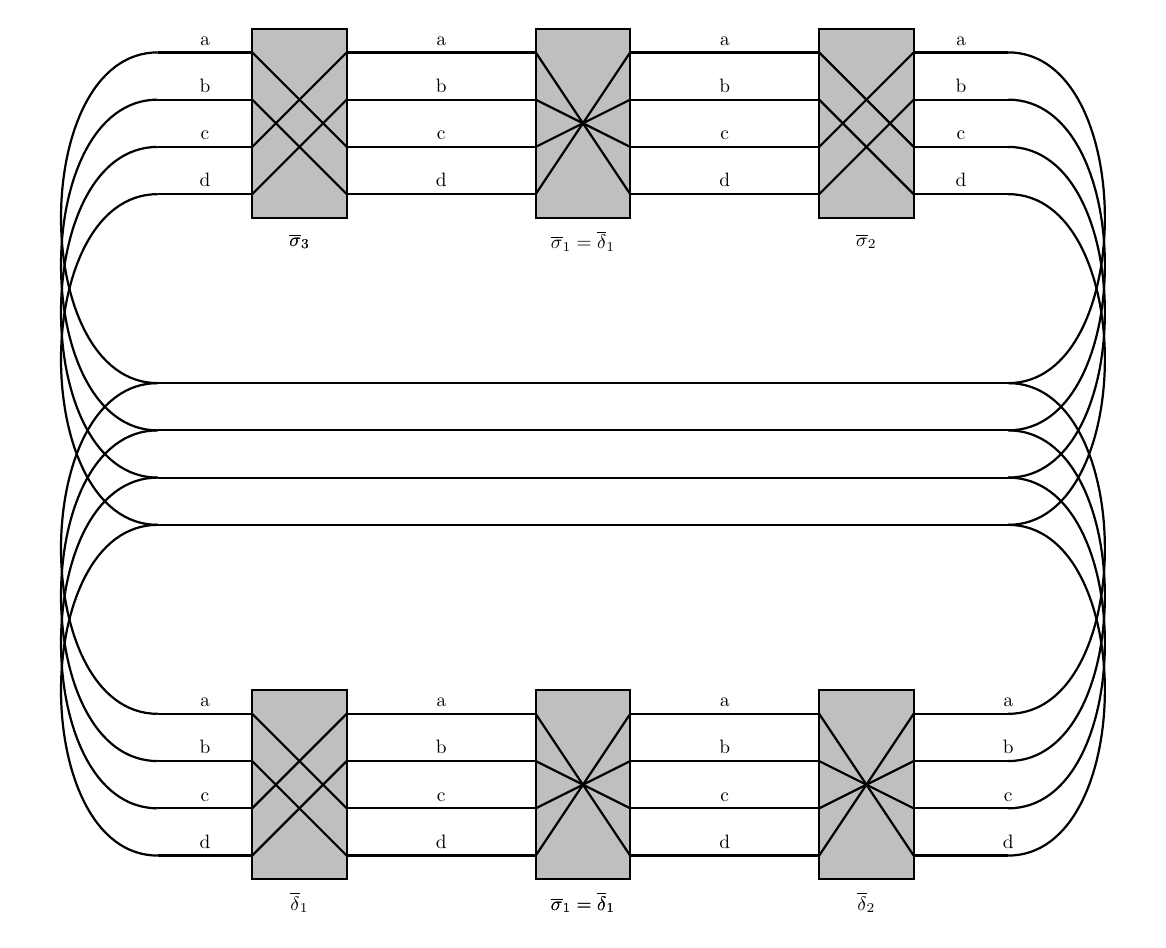
\begin{tikzpicture}[thick, scale=0.6, every node/.style={scale=0.7}]
            % Draw the box
            \draw[fill=lightgray] (2-6,-1.5) rectangle (4-6,2.5) node[midway] {};
            
            \node at (3-6, -2) {$\overline\sigma_3$};

            % Draw the wires entering the box
            \draw[-] (0-6, 2) -- (2-6, 2) node[midway, above] {a};
            \draw[-] (0-6, 1) -- (2-6, 1) node[midway, above] {b};
            \draw[-] (0-6, 0) -- (2-6, 0) node[midway, above] {c};
            \draw[-] (0-6,-1) -- (2-6,-1) node[midway, above] {d};

            % Draw the wires exiting the box with crossed mappings
            \draw[-] (4-6, 2) -- (6-6,2) node[right, above] {a};
            \draw[-] (4-6, 1) -- (6-6, 1) node[right, above] {b};
            \draw[-] (4-6, 0) -- (6-6, 0) node[right, above] {c};
            \draw[-] (4-6,-1) -- (6-6, -1) node[right, above] {d};

            % Draw the lines inside the box to represent the mapping
            \draw[-] (2-6, 2) -- (4-6,0);
            \draw[-] (2-6, 1) -- (4-6, -1);
            \draw[-] (2-6, 0) -- (4-6, 2);
            \draw[-] (2-6,-1) -- (4-6, 1);

            \draw[fill=lightgray] (2,-1.5) rectangle (4,2.5) node[midway] {};

            \node at (3, -2) {$\overline\sigma_1 = \overline\delta_1$};

            % Draw the wires entering the box
            \draw[-] (0, 2) -- (2, 2) node[midway, above] {};
            \draw[-] (0, 1) -- (2, 1) node[midway, above] {};
            \draw[-] (0, 0) -- (2, 0) node[midway, above] {};
            \draw[-] (0,-1) -- (2,-1) node[midway, above] {};

            % Draw the wires exiting the box
            \draw[-] (4, 2) -- (6,2) node[right, above] {a};
            \draw[-] (4, 1) -- (6, 1) node[right, above] {b};
            \draw[-] (4, 0) -- (6, 0) node[right, above] {c};
            \draw[-] (4,-1) -- (6, -1) node[right, above] {d};

            % Draw the lines inside the box to represent the mapping
            \draw[-] (2, 2) -- (4, -1);
            \draw[-] (2, 1) -- (4, 0);
            \draw[-] (2, 0) -- (4, 1);
            \draw[-] (2,-1) -- (4, 2);

            \draw[fill=lightgray] (2+6,-1.5) rectangle (4+6,2.5) node[midway] {};
            
            \node at (3+6, -2) {$\overline\sigma_2$};


            % Draw the wires entering the box
            \draw[-] (0+6, 2) -- (2+6, 2) node[midway, above] {};
            \draw[-] (0+6, 1) -- (2+6, 1) node[midway, above] {};
            \draw[-] (0+6, 0) -- (2+6, 0) node[midway, above] {};
            \draw[-] (0+6,-1) -- (2+6,-1) node[midway, above] {};

            % Draw the wires exiting the box
            \draw[-] (4+6, 2) -- (6+6,2) node[midway, above] {a};
            \draw[-] (4+6, 1) -- (6+6, 1) node[midway, above] {b};
            \draw[-] (4+6, 0) -- (6+6, 0) node[midway, above] {c};
            \draw[-] (4+6,-1) -- (6+6, -1) node[midway, above] {d};

            \draw[-] (2+6, 2) -- (4+6, 0);
            \draw[-] (2+6, 1) -- (4+6, -1);
            \draw[-] (2+6, 0) -- (4+6, 2);
            \draw[-] (2+6,-1) -- (4+6, 1);

            \draw[-] (0-6, 2) to[out=180, in=180] (-6, 2-7) node[midway, above] {};
            \draw[-] (0-6, 1) to[out=180, in=180] (-6, 1-7) node[midway, above] {};
            \draw[-] (0-6, 0) to[out=180, in=180] (-6, 0-7) node[midway, above] {};
            \draw[-] (0-6, -1) to[out=180, in=180] (-6, -1-7) node[midway, above] {};

            \draw[-] (6+6, 2) to[out=360, in=360] (6+6, 2-7) node[midway, above] {};
            \draw[-] (6+6, 1) to[out=360, in=360] (6+6, 1-7) node[midway, above] {};
            \draw[-] (6+6, 0) to[out=360, in=360] (6+6, 0-7) node[midway, above] {};
            \draw[-] (6+6, -1) to[out=360, in=360] (6+6, -1-7) node[midway, above] {};

            \draw[-] (-6, 2-7) to (6+6, 2-7) node[midway, above] {};
            \draw[-] (-6, 1-7) to (6+6, 1-7) node[midway, above] {};
            \draw[-] (-6, 0-7) to (6+6, 0-7) node[midway, above] {};
            \draw[-] (-6, -1-7) to (6+6, -1-7) node[midway, above] {};

            \draw[-] (0-6, 2-14) to[out=180, in=180] (-6, 2-7) node[midway, above] {};
            \draw[-] (0-6, 1-14) to[out=180, in=180] (-6, 1-7) node[midway, above] {};
            \draw[-] (0-6, 0-14) to[out=180, in=180] (-6, 0-7) node[midway, above] {};
            \draw[-] (0-6, -1-14) to[out=180, in=180] (-6, -1-7) node[midway, above] {};

            \draw[-] (6+6, 2-14) to[out=360, in=360] (6+6, 2-7) node[midway, above] {};
            \draw[-] (6+6, 1-14) to[out=360, in=360] (6+6, 1-7) node[midway, above] {};
            \draw[-] (6+6, 0-14) to[out=360, in=360] (6+6, 0-7) node[midway, above] {};
            \draw[-] (6+6, -1-14) to[out=360, in=360] (6+6, -1-7) node[midway, above] {};

            \draw[fill=lightgray] (2-6,-1.5-14) rectangle (4-6,2.5-14) node[midway] {};
            
            \node at (3-6, -2) {$\overline\sigma_3$};

            % Draw the wires entering the box
            \draw[-] (0-6, 2-14) -- (2-6, 2-14) node[midway, above] {a};
            \draw[-] (0-6, 1-14) -- (2-6, 1-14) node[midway, above] {b};
            \draw[-] (0-6, 0-14) -- (2-6, 0-14) node[midway, above] {c};
            \draw[-] (0-6,-1-14) -- (2-6,-1-14) node[midway, above] {d};

            % Draw the wires exiting the box with crossed mappings
            \draw[-] (4-6, 2-14) -- (6-6,2-14) node[right, above] {a};
            \draw[-] (4-6, 1-14) -- (6-6, 1-14) node[right, above] {b};
            \draw[-] (4-6, 0-14) -- (6-6, 0-14) node[right, above] {c};
            \draw[-] (4-6,-1-14) -- (6-6, -1-14) node[right, above] {d};

            % Draw the lines inside the box to represent the mapping
            \draw[-] (2-6, 2-14) -- (4-6,0-14);
            \draw[-] (2-6, 1-14) -- (4-6, -1-14);
            \draw[-] (2-6, 0-14) -- (4-6, 2-14);
            \draw[-] (2-6,-1-14) -- (4-6, 1-14);

            \node at (3-6, -2-14) {$\overline\delta_1$};

            \draw[fill=lightgray] (2,-1.5-14) rectangle (4,2.5-14) node[midway] {};

            \node at (3, -2-14) {$\overline\sigma_1 = \overline\delta_1$};

            % Draw the wires entering the box
            \draw[-] (0, 2-14) -- (2, 2-14) node[midway, above] {};
            \draw[-] (0, 1-14) -- (2, 1-14) node[midway, above] {};
            \draw[-] (0, 0-14) -- (2, 0-14) node[midway, above] {};
            \draw[-] (0,-1-14) -- (2,-1-14) node[midway, above] {};

            % Draw the wires exiting the box
            \draw[-] (4, 2-14) -- (6,2-14) node[right, above] {a};
            \draw[-] (4, 1-14) -- (6, 1-14) node[right, above] {b};
            \draw[-] (4, 0-14) -- (6, 0-14) node[right, above] {c};
            \draw[-] (4,-1-14) -- (6, -1-14) node[right, above] {d};

            % Draw the lines inside the box to represent the mapping
            \draw[-] (2, 2-14) -- (4, -1-14);
            \draw[-] (2, 1-14) -- (4, 0-14);
            \draw[-] (2, 0-14) -- (4, 1-14);
            \draw[-] (2,-1-14) -- (4, 2-14);

            \draw[fill=lightgray] (2+6,-1.5-14) rectangle (4+6,2.5-14) node[midway] {};

            \node at (3, -2-14) {$\overline\sigma_1 = \overline\delta_1$};

            % Draw the wires entering the box
            \draw[-] (0+6, 2-14) -- (2+6, 2-14) node[midway, above] {};
            \draw[-] (0+6, 1-14) -- (2+6, 1-14) node[midway, above] {};
            \draw[-] (0+6, 0-14) -- (2+6, 0-14) node[midway, above] {};
            \draw[-] (0+6,-1-14) -- (2+6,-1-14) node[midway, above] {};

            % Draw the wires exiting the box
            \draw[-] (4+6, 2-14) -- (6+6,2-14) node[right, above] {a};
            \draw[-] (4+6, 1-14) -- (6+6, 1-14) node[right, above] {b};
            \draw[-] (4+6, 0-14) -- (6+6, 0-14) node[right, above] {c};
            \draw[-] (4+6,-1-14) -- (6+6, -1-14) node[right, above] {d};

            % Draw the lines inside the box to represent the mapping
            \draw[-] (2+6, 2-14) -- (4+6, -1-14);
            \draw[-] (2+6, 1-14) -- (4+6, 0-14);
            \draw[-] (2+6, 0-14) -- (4+6, 1-14);
            \draw[-] (2+6,-1-14) -- (4+6, 2-14);

            \node at (3+6, -2-14) {$\overline\delta_2$};
            % \node[draw,circle] at (-4.5, -1) {$A$};
            % \node[draw,circle] at (3, -9) {$B$};
            % \node[draw,circle] at (10.5, -1) {$C$};
        \end{tikzpicture}
    \end{center}